% !TEX program = lualatex
% Compile from 2026/week10; figures are reproduced by make_figures.py.
\documentclass[12pt,aspectratio=43]{beamer}
% Shared Beamer design. Load after \documentclass using \input.
% Engine: LuaLaTeX. Fonts: UD Digi Kyokasho N (regular/bold), Arial.
\usepackage{luatexja-fontspec}
\setmainjfont[BoldFont={UD Digi Kyokasho N Bold}]{UD Digi Kyokasho N}
\setsansjfont[BoldFont={UD Digi Kyokasho N Bold}]{UD Digi Kyokasho N}
\setmonojfont[BoldFont={UD Digi Kyokasho N Bold}]{UD Digi Kyokasho N}
% Liberation Sans keeps the layout usable on systems without Arial.
\IfFontExistsTF{Arial}{
  \setmainfont{Arial}
  \setsansfont{Arial}
  \setmonofont{Arial}
}{
  \setmainfont{Liberation Sans}
  \setsansfont{Liberation Sans}
  \setmonofont{Liberation Sans}
}
\renewcommand{\kanjifamilydefault}{\gtdefault}

% Typeset mathematics with a dedicated TeX math font, independent of Arial.
\usefonttheme{professionalfonts}
\usepackage[mathrm=sym]{unicode-math}
\setmathfont{Latin Modern Math}
\setoperatorfont{\symup}

\definecolor{courseblue}{HTML}{4472C4}
\definecolor{ruleblue}{HTML}{8FAADC}
\setbeamercolor{normal text}{fg=black,bg=white}
\setbeamercolor{structure}{fg=courseblue}
\setbeamercolor{frametitle}{fg=black,bg=white}
\setbeamercolor{title banner}{fg=white,bg=courseblue}
\setbeamerfont{frametitle}{size=\fontsize{18}{22}\selectfont,series=\mdseries}
\setbeamerfont{quote}{shape=\upshape}
\setbeamersize{text margin left=9mm,text margin right=9mm}
\setbeamertemplate{navigation symbols}{}
\setbeamercolor{page number}{fg=gray,bg=white}
\setbeamertemplate{footline}{%
  \begin{beamercolorbox}[wd=\paperwidth,ht=2.5mm,dp=1.5mm]{page number}
    \hfill{\fontsize{8}{9}\selectfont
      \ifnum\value{framenumber}>0
        \insertframenumber\,/\,\inserttotalframenumber
      \fi}\hspace*{3mm}
  \end{beamercolorbox}}
\setbeamertemplate{headline}{%
  \hfill\textcolor{gray}{\fontsize{6}{7}\selectfont
    \hypersetup{linkcolor=gray}% Keep Beamer's title links in the header color.
    \ifnum\value{framenumber}=0 \insertshortdate\enspace\fi
    \insertshorttitle\space\insertshortsubtitle}\hspace{2mm}\vspace{1.5mm}}
\setbeamertemplate{frametitle}{%
  \vspace{2mm}\centering\insertframetitle\par
  \vspace{-1mm}{\color{ruleblue}\rule{.44\paperwidth}{.5pt}}\par
  \vspace{2mm}}
\setbeamercolor{itemize item}{fg=courseblue}
\setbeamercolor{itemize subitem}{fg=black}
\setbeamercolor{itemize subsubitem}{fg=black}
\setbeamertemplate{itemize item}{\textbullet}
\setbeamertemplate{itemize subitem}{\textnormal{-}}
\setbeamertemplate{itemize subsubitem}{\textnormal{-}}
\setlength{\parskip}{.45em}
\hypersetup{colorlinks=true,urlcolor=courseblue}

% Use \titlepage inside a [t,noframenumbering] frame. The background extends
% 1 mm past both page edges to avoid hairline gaps in PDF viewers.
\setbeamertemplate{title page}{%
  \vspace{2mm}
  \begin{beamercolorbox}[wd=\paperwidth,ht=43mm,dp=13mm,colsep*=1mm,center]{title banner}
    {\fontsize{32}{40}\selectfont\inserttitle\par}
    \vspace{2mm}
    {\fontsize{20}{24}\selectfont\insertsubtitle\par}
  \end{beamercolorbox}
  \vspace{10mm}
  \hfill\insertauthor
}

\graphicspath{{figures/}}
\usepackage{listings}
\usepackage{upquote}
\IfFontExistsTF{Consolas}{\newfontfamily\codefont{Consolas}}{\newfontfamily\codefont{Liberation Mono}}
\definecolor{codevalue}{HTML}{7A3E9D}
\definecolor{codebuiltin}{HTML}{006DB0}
\definecolor{codestring}{HTML}{267348}
\newcommand{\code}[1]{{\codefont #1}}
\lstdefinestyle{python}{
  language=Python,
  basicstyle=\codefont\fontsize{12}{14}\selectfont,
  keywordstyle=\color{codebuiltin},
  keywordstyle=[2]\color{codebuiltin},
  morekeywords=[2]{print,range},
  stringstyle=\color{codestring},
  showstringspaces=false,
  columns=fullflexible,
  keepspaces=true,
  upquote=true,
  tabsize=4,
  breaklines=false,
  backgroundcolor=\color{black!4},
  frame=single,framerule=0pt,framesep=1.7mm,
  xleftmargin=1.7mm,xrightmargin=1.7mm,
  aboveskip=1mm,belowskip=0.5mm,
  literate=*{0}{{{\color{codevalue}0}}}1
    {1}{{{\color{codevalue}1}}}1 {2}{{{\color{codevalue}2}}}1
    {3}{{{\color{codevalue}3}}}1 {4}{{{\color{codevalue}4}}}1
    {5}{{{\color{codevalue}5}}}1 {6}{{{\color{codevalue}6}}}1
    {7}{{{\color{codevalue}7}}}1 {8}{{{\color{codevalue}8}}}1
    {9}{{{\color{codevalue}9}}}1
}
\lstset{style=python}
\setbeamercolor{lesson note}{fg=black,bg=courseblue!9}
\newenvironment{lessonbox}
  {\begin{beamercolorbox}[wd=\linewidth,sep=1.5mm]{lesson note}}
  {\end{beamercolorbox}\par}

\title{計算物理学B}
\subtitle{第十回：常微分方程式1}
\author{野垣 康介、藤本 悠輝}
\date{2026/12/22}
\hypersetup{pdftitle={計算物理学B 第十回：常微分方程式1},pdfauthor={野垣 康介、藤本 悠輝}}

\begin{document}

\begin{frame}[t,noframenumbering]
  \titlepage
\end{frame}

\begin{frame}[t]{講義予定}
  \begingroup
  \setlength{\tabcolsep}{1.6mm}
  \renewcommand{\arraystretch}{1.25}
  \begin{tabular}{@{}l@{\hspace{2mm}}l@{\hspace{4mm}}l@{\hspace{2mm}}l@{}}
    10/6 & 四則演算 & 12/8 & モンテカルロ1 \\
    10/27 & 制御文（for, if） & 12/15 & モンテカルロ2 \\
    11/6（金） & 関数 & \textcolor{courseblue}{\textbf{12/22}} &
      \textcolor{courseblue}{\textbf{微分方程式1}} \\
    11/10 & 配列（NumPy） & 1/12 & 微分方程式2 \\
    11/17 & 可視化（matplotlib） & 1/19 & 偏微分方程式1 \\
    11/24 & 数値微分 & 1/26 & 偏微分方程式2 \\
    12/1 & 数値積分 & 2/2 & 根の探索 \\
    \multicolumn{2}{c}{\small 〜中間レポート〜} &
    \multicolumn{2}{c}{\small 〜期末レポート〜}
  \end{tabular}\par
  \endgroup
  \vspace{2mm}
  {\small 10/20は出張で休講。11/6（金）は火曜授業の振替。\par}
\end{frame}

\begin{frame}[t]{今日の内容}
  \begin{itemize}
    \setlength{\itemsep}{2.5mm}
    \item Euler法、Runge--Kutta法（RK2・RK4）
    \item 連立1階方程式と2階運動方程式
    \item 陽解法・陰解法と硬い方程式
    \item 適応刻み幅制御と単振り子の実習
  \end{itemize}
\end{frame}

\begin{frame}[t]{Notebookを開く}
  \begin{itemize}
    \setlength{\itemsep}{2.5mm}
    \item Google Colab：\small\url{https://colab.research.google.com/?hl=ja}
    \item GitHub：\small\href{https://github.com/nogaki/Computational_Physics_B/tree/main/2026/week10/week10.ipynb}{2026/week10/week10.ipynb}
    \item Colabの「ファイル」\(\to\)「ノートブックを開く」\(\to\)「GitHub」から開く
  \end{itemize}
  \vspace{2mm}
  \begin{lessonbox}
    \textbf{開いたら「ドライブにコピーを保存」}\par
    \small 開いただけでは自分のDriveに保存されません。セルを先頭から順に実行します。
  \end{lessonbox}
\end{frame}

\begin{frame}[t]{常微分方程式の初期値問題}
  1階常微分方程式（ODE）の初期値問題は
  \[
    \frac{dx}{dt}=f(x,t),\qquad x(t_0)=x_0
  \]
  であり、解 $x(t)$ の時間発展を求める。
  \[
    x(t)=x_0+\int_{t_0}^{t} f(x(t'),t')\,dt'
  \]
  \begin{itemize}
    \setlength{\itemsep}{1mm}
    \item 力学では $t$ は時間だが、一般の独立変数でもよい
    \item 解析積分ができない問題でも、刻み幅ごとに近似できる
  \end{itemize}
\end{frame}

\begin{frame}[t]{基本的な数値解法と誤差}
  \begin{center}
  \renewcommand{\arraystretch}{1.5}
  \begin{tabular}{lcc}
    \hline
    方法 & 1ステップの局所誤差 & 大域誤差 \\
    \hline
    Euler & $\mathcal{O}(h^2)$ & $\mathcal{O}(h)$ \\
    RK2 & $\mathcal{O}(h^3)$ & $\mathcal{O}(h^2)$ \\
    RK4 & $\mathcal{O}(h^5)$ & $\mathcal{O}(h^4)$ \\
    \hline
  \end{tabular}
  \end{center}
  \small 局所誤差は1ステップで生じる誤差。大域誤差は有限時間積分後に蓄積した誤差。
  滑らかな解と安定な計算を仮定した次数。
\end{frame}

\begin{frame}[t]{Euler法}
  Taylor展開を1次まで使うと
  \[
    x(t+h)=x(t)+h\frac{dx}{dt}+\mathcal{O}(h^2).
  \]
  $dx/dt=f(x,t)$ を代入して高次項を捨てる。
  \[
    x_{n+1}=x_n+h f(x_n,t_n)
  \]
  \begin{itemize}
    \setlength{\itemsep}{1mm}
    \item 毎ステップで始点の傾きを使う陽解法
    \item 大域誤差は刻み幅 $h$ に比例する
  \end{itemize}
\end{frame}

\begin{frame}[t]{刻み幅を変える}
  \centering
  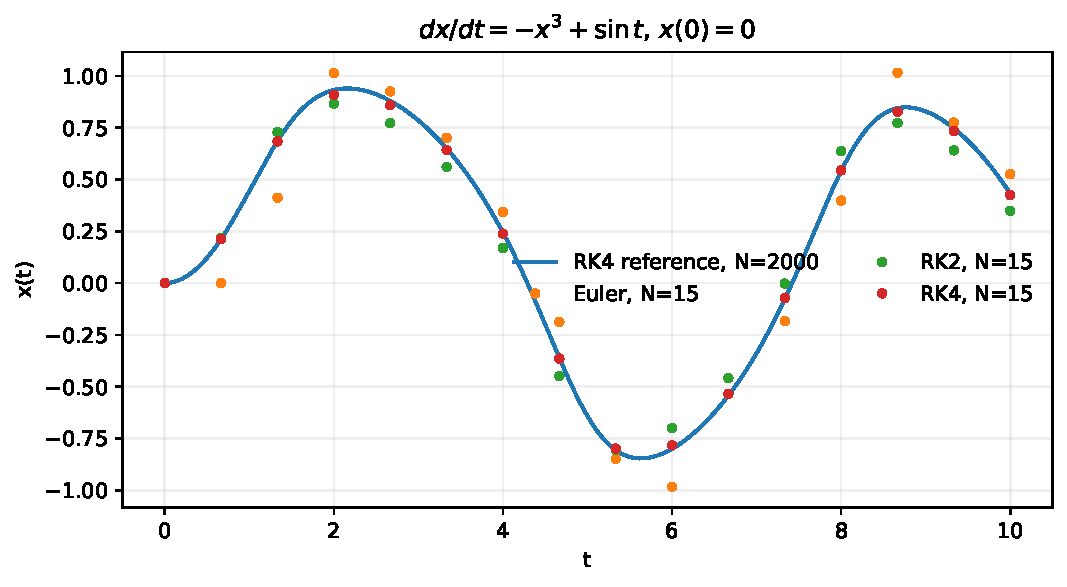
\includegraphics[width=0.78\linewidth]{ode_methods.pdf}

  \small $dx/dt=-x^3+\sin t$、$x(0)=0$。
  N=15の各手法を、RK4・N=2000の数値解と比較。
\end{frame}

\begin{frame}[t]{中点法：2次Runge--Kutta法}
  始点の傾きと、その傾きで予測した中点の傾きを使う。
  \[
    \begin{aligned}
      k_1&=h f(x_n,t_n),\\
      k_2&=h f(x_n+k_1/2,t_n+h/2),\\
      x_{n+1}&=x_n+k_2.
    \end{aligned}
  \]
  \begin{itemize}
    \setlength{\itemsep}{1.5mm}
    \item 中点で傾きを評価する
    \item 局所誤差 $\mathcal{O}(h^3)$、大域誤差 $\mathcal{O}(h^2)$
  \end{itemize}
\end{frame}

\begin{frame}[t]{4次Runge--Kutta法}
  始点、中点2回、終点で傾きを評価し、重み付けして平均する。
  \[
    \begin{aligned}
      k_1&=h f(x_n,t_n),\\
      k_2&=h f(x_n+k_1/2,t_n+h/2),\\
      k_3&=h f(x_n+k_2/2,t_n+h/2),\\
      k_4&=h f(x_n+k_3,t_n+h),\\
      x_{n+1}&=x_n+(k_1+2k_2+2k_3+k_4)/6.
    \end{aligned}
  \]
  \begin{itemize}
    \setlength{\itemsep}{1mm}
    \item 局所誤差 $\mathcal{O}(h^5)$、大域誤差 $\mathcal{O}(h^4)$
    \item 物理系の初期値問題でよく使われる陽解法
  \end{itemize}
\end{frame}

\begin{frame}[t]{刻み幅と大域誤差}
  \centering
  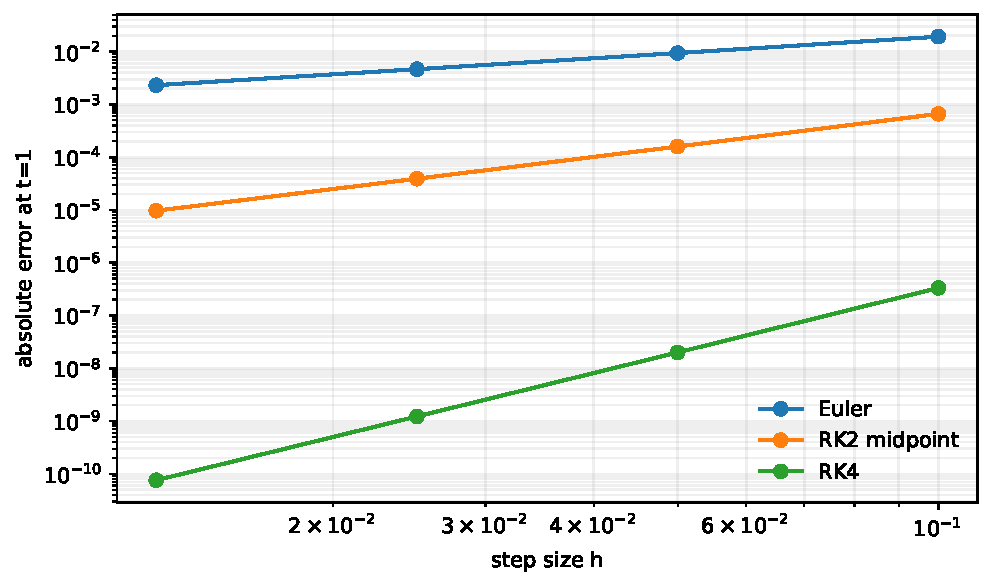
\includegraphics[width=0.73\linewidth]{ode_order.pdf}

  \small $x'=-x$、$x(0)=1$ を $t=1$ まで解き、厳密解と比較。
  誤差が $h$ の何乗で減るかを対数軸で示す。
\end{frame}

\begin{frame}[t]{連立1階常微分方程式}
  $N$変数の連立系をベクトルでまとめる。
  \[
    \frac{dx_i}{dt}=f_i(x_1,\ldots,x_N,t),\qquad
    \frac{d\mathbf{x}}{dt}=\mathbf{f}(\mathbf{x},t)
  \]
  Euler法・RK2法・RK4法はベクトルの各成分に同じ形で適用できる。
  \begin{lessonbox}
    例：$\dot{x}=xy-x$、
    $\dot{y}=y-xy+\sin^2 t$。状態を
    $\mathbf{x}=(x,y)$ として一度に更新する。
  \end{lessonbox}
\end{frame}

\begin{frame}[t,fragile]{2階の運動方程式}
  $N$個の一般化座標を含む2階方程式
  \[
    \frac{d^2\mathbf{q}}{dt^2}
      =\mathbf{F}(\mathbf{q},d\mathbf{q}/dt,t)
  \]
  に対し、速度 $\mathbf{v}=d\mathbf{q}/dt$ を導入する。
  \[
    \frac{d}{dt}\begin{pmatrix}\mathbf{q}\\\mathbf{v}\end{pmatrix}
      =\begin{pmatrix}\mathbf{v}\\\mathbf{F}(\mathbf{q},\mathbf{v},t)\end{pmatrix}
  \]
  \begin{lessonbox}
    $2N$元の1階連立ODEになり、これまでの積分法をそのまま使える。
  \end{lessonbox}
\end{frame}

\begin{frame}[t]{実習：単振り子}
  \begin{columns}[T,onlytextwidth]
    \column{0.58\textwidth}
    支点まわりの運動方程式は
    \[
      \begin{aligned}
        mL^2\ddot{\theta}&=-mgL\sin\theta,\\
        \ddot{\theta}&=-\frac{g}{L}\sin\theta.
      \end{aligned}
    \]
    \begin{itemize}
      \setlength{\itemsep}{1mm}
      \item $\omega=\dot{\theta}$ として1階系に直す
      \item $g=9.81\,\mathrm{m/s^2}$、$L=0.1\,\mathrm{m}$
      \item 小角近似と数値解を比べる
    \end{itemize}
    \column{0.39\textwidth}
    \centering
    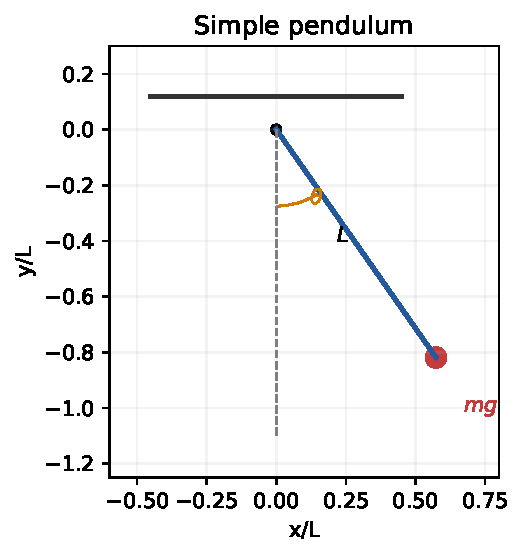
\includegraphics[width=\linewidth]{pendulum_scheme.pdf}
  \end{columns}
  \[
    \theta(t)\simeq\theta_0\cos\!\left(\sqrt{g/L}\,t\right)
    \quad (|\theta_0|\ll1,\ \dot\theta(0)=0)
  \]
\end{frame}

\begin{frame}[t]{陽解法と陰解法}
  \begin{columns}[T,onlytextwidth]
    \column{0.48\textwidth}
    \textbf{前進Euler法（陽）}
    \[
      x_{n+1}=x_n+h f(x_n,t_n)
    \]
    既知の値 $x_n$ だけで次の値を計算。
    \column{0.48\textwidth}
    \textbf{後退Euler法（陰）}
    \[
      x_{n+1}=x_n+h f(x_{n+1},t_{n+1})
    \]
    次の値を含む方程式を解いて更新。
  \end{columns}
  \vspace{3mm}
  \begin{itemize}
    \setlength{\itemsep}{1mm}
    \item 陽解法は簡単だが、刻み幅に安定性の制限がある
    \item 陰解法は各ステップの計算が増えるが、硬い系で安定になりやすい
  \end{itemize}
\end{frame}

\begin{frame}[t]{硬い方程式の例}
  \[
    \frac{dx}{dt}=-cx,\quad c\gg1,\quad x(0)=1,
    \qquad x(t)=e^{-ct}.
  \]
  短い時間で急減衰する。陽Euler法は
  \[
    x_{n+1}=(1-ch)x_n.
  \]
  数値解が減衰するには
  \[
    |1-ch|<1\quad\Longleftrightarrow\quad 0<h<\frac{2}{c}.
  \]
  \small 安定性は数値誤差が増幅しない条件。解析解への近さ（精度）とは別。
\end{frame}

\begin{frame}[t]{硬い方程式：陽Euler法}
  \centering
  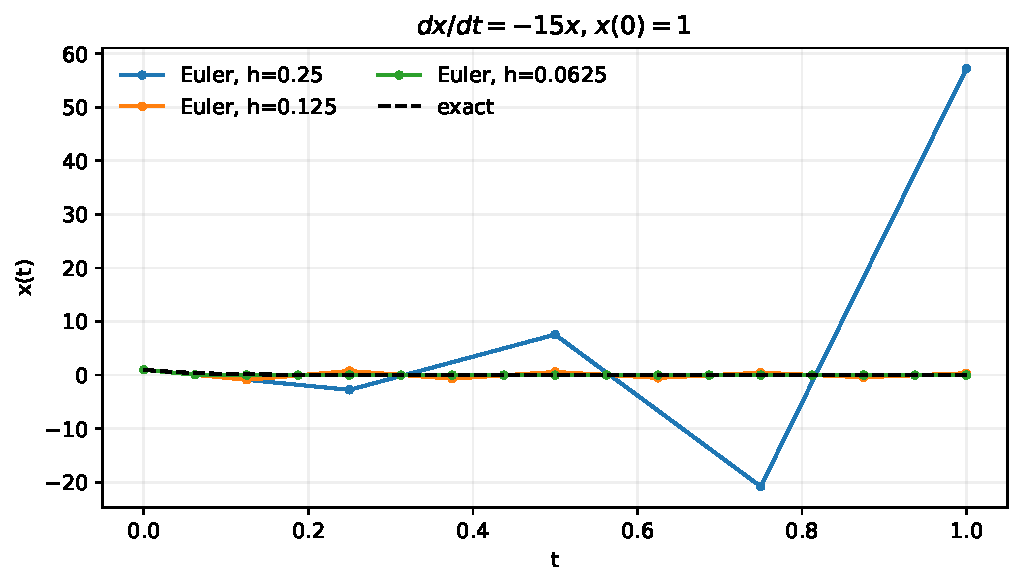
\includegraphics[width=0.78\linewidth]{stiff_euler.pdf}

  \small $c=15$、$0\le t\le1$。$h=1/4$ は安定条件を満たさず、数値解が発散する。
\end{frame}

\begin{frame}[t]{硬い方程式：RK4法}
  \centering
  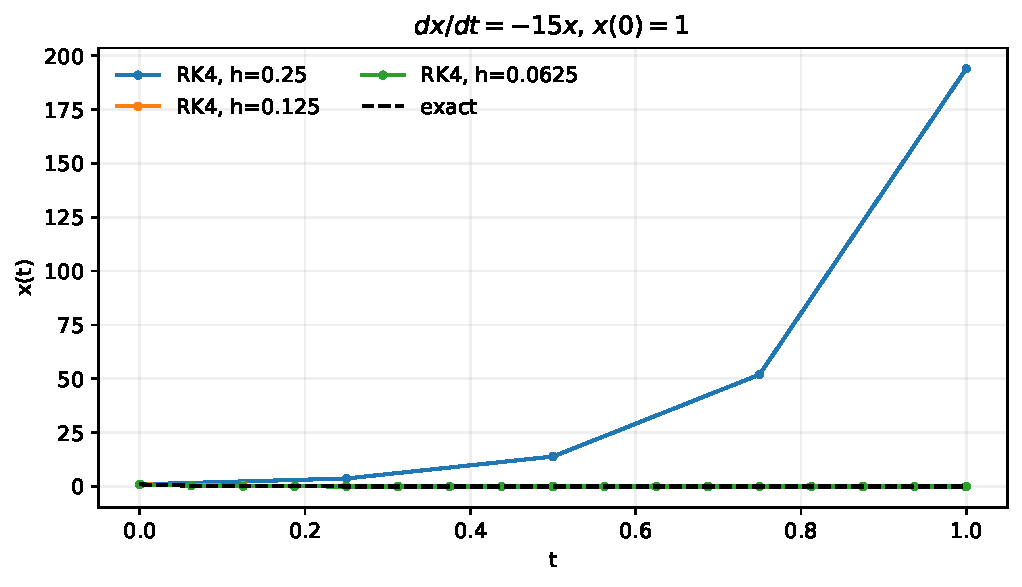
\includegraphics[width=0.78\linewidth]{stiff_rk4.pdf}

  \small 高次法でも安定条件がある。$h=1/4$ ではこの問題に対して発散する。
\end{frame}

\begin{frame}[t]{後退Euler法の安定性}
  硬い方程式 $\dot{x}=-cx$ に代入すると
  \[
    x_{n+1}=\frac{x_n}{1+ch}.
  \]
  \begin{itemize}
    \setlength{\itemsep}{1.5mm}
    \item $c,h>0$ なら増幅率 $1/(1+ch)$ は0と1の間
    \item どの正の $h$ でも解は発散しない
    \item 大きな $h$ では安定でも精度は悪くなり得る
  \end{itemize}
\end{frame}

\begin{frame}[t]{硬い方程式：陰Euler法}
  \centering
  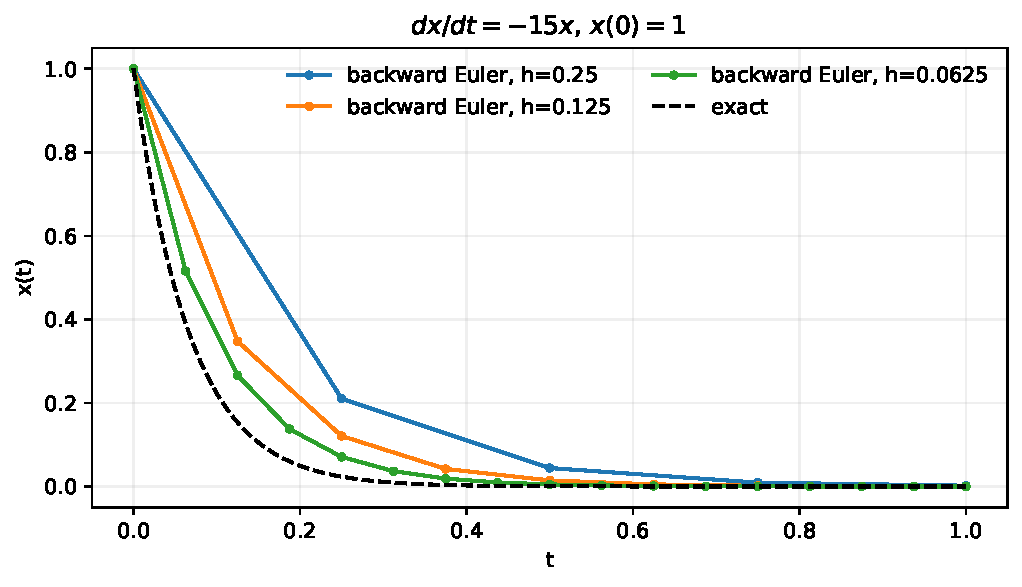
\includegraphics[width=0.78\linewidth]{stiff_backward.pdf}

  \small 全ての刻み幅で数値解は安定。ただし大きな刻み幅では厳密解の急減衰を捉えない。
\end{frame}

\begin{frame}[t]{適応刻み幅制御}
  RK4の刻み幅 $h$ を1回使う解と、$h/2$ を2回使う解を比べる。
  \[
    e\simeq\frac{|x_{h/2}^{(2)}-x_h|}{2^4-1}
      =\frac{|x_{h/2}^{(2)}-x_h|}{15}
  \]
  \begin{itemize}
    \setlength{\itemsep}{1.5mm}
    \item 誤差が許容値より大きければ刻み幅を縮めて再計算
    \item 十分小さければ2つの半ステップ解を採用
    \item 誤差が $h^5$ に比例するので刻み幅更新は5乗根に比例
  \end{itemize}
  \small ここでは局所絶対誤差を使う。相対誤差を含む制御はSciPyのソルバーで扱う。
\end{frame}

\begin{frame}[t]{適応刻み幅の例}
  \centering
  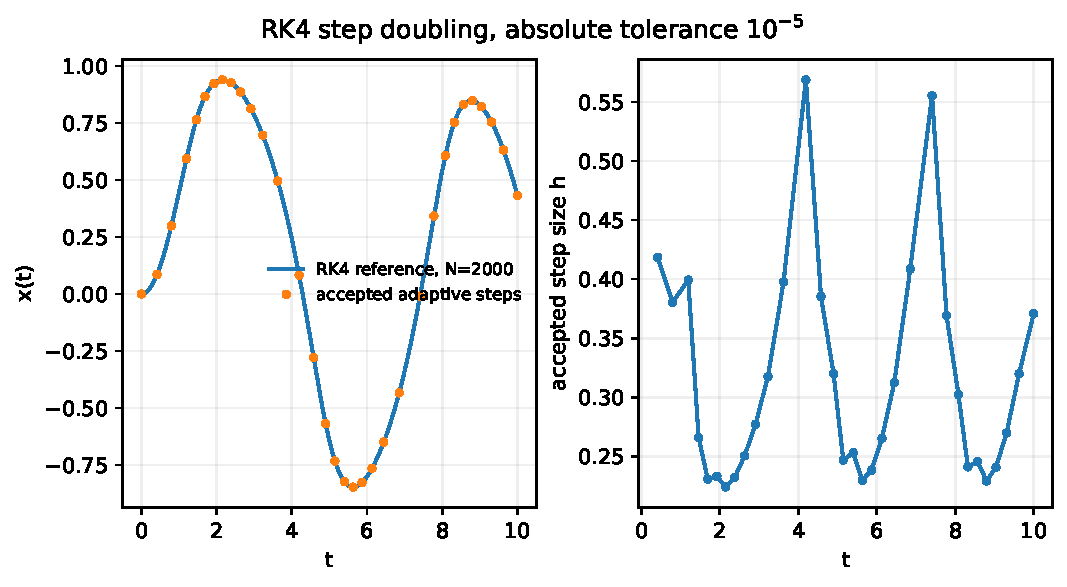
\includegraphics[width=0.86\linewidth]{adaptive_rk4.pdf}

  \small 左：一定刻み幅の参照解と採用点。右：推定誤差に応じて変わる刻み幅。
\end{frame}

\begin{frame}[t,fragile]{SciPyのsolve\_ivp}
  実用ではSciPyの初期値問題ソルバーも使える。
  右辺関数は \code{fun(t, y)} の順に引数を取る。
  \begin{lstlisting}
from scipy.integrate import solve_ivp
sol = solve_ivp(fun, (0.0, 10.0), [0.0],
                rtol=1e-8, atol=1e-10)
if sol.success:
    print(sol.t[-1], sol.y[0, -1])
  \end{lstlisting}
  \begin{lessonbox}
    返り値の成功状態と許容誤差を確認する。数値手法の性質を知ると、
    ソルバー選択と結果の確認がしやすい。
  \end{lessonbox}
\end{frame}

\begin{frame}[t]{実習タイム}
  \begin{enumerate}
    \setlength{\itemsep}{2.5mm}
    \item 単振り子の方程式を$(\theta,\omega)$の1階系に直す
    \item RK4で $0\le t\le2\,\mathrm{s}$ を解く
    \item 小角近似 $\theta_0\cos(\sqrt{g/L}\,t)$ と比較する
    \item 初期角を変え、近似が成り立つ範囲を確かめる
  \end{enumerate}
  \vspace{2mm}
  \small Notebookの最後に解答用セルを残しています。
\end{frame}

\end{document}
